
\begin{figure}[t]
\centering
\begin{tikzpicture}
    \begin{customlegend}[legend columns=4,
        legend entries={\sketragp, \sketragu, \skeletonrag\eat{, \skeletonragu}}
        ,
        legend style={at={(0.45,1.05)},anchor=north,draw=none,font=\footnotesize,column sep=0.1cm}]
    \addlegendimage{line width=0.3mm,mark size=2pt,mark=o,color=Red}
    \addlegendimage{line width=0.3mm,mark size=2pt,mark=x,color=Orange}
    \addlegendimage{line width=0.3mm,mark size=2pt,mark=triangle,color=LightBlue}
    % \addlegendimage{line width=0.3mm,mark size=2pt,mark=star,color=DeepBlue}
    \end{customlegend}
\end{tikzpicture}
% \vspace{-2mm}
\\
\subfloat[MuSiQue]{
\hspace{-1.2mm}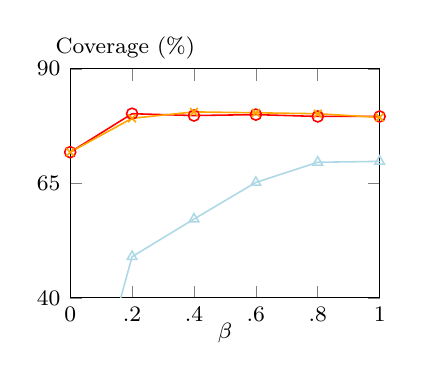
\begin{tikzpicture}[scale=1]
    \begin{axis}[
        height=\columnwidth/2.7,
        width=\columnwidth/2.2,
        ylabel={Coverage (\%)},
        xlabel={$\beta$},
        xmin=0.0, xmax=1.0,
        ymin=0.4, ymax=0.9,
        xtick={0, 0.2, 0.4, 0.6, 0.8, 1.0},
        xticklabel style = {font=\footnotesize},
        xticklabels={0, .2, .4, .6, .8, 1},
        ytick={0.4, 0.65, 0.9},
        yticklabels={40, 65, 90},
        every axis y label/.style={at={(current axis.north west)},right=7mm,above=0mm},
        label style={font=\footnotesize},
        tick label style={font=\footnotesize},
        every axis x label/.style={at={(current axis.south)},right=0mm,above=-7mm},
        label style={font=\footnotesize},
        tick label style={font=\footnotesize},
    ]

%     \addplot[line width=0.2mm,mark size=2pt,mark=o,color=Red]
%         plot coordinates { % SkeTRAG - 1200
% (0, 0.176300934)
% (0.2, 0.188094157)
% (0.4, 0.196128801)
% (0.6, 0.1876783)
% (0.8, 0.19700453)
% (1.0, 0.157561628)
%     };

%     \addplot[line width=0.2mm,mark size=2pt,mark=o,color=Red!75]
%         plot coordinates { % SkeTRAG - 600
% (0, 0.170179462)
% (0.2, 0.240968426)
% (0.4, 0.226319961)
% (0.6, 0.232188549)
% (0.8, 0.229216351)
% (1.0, 0.208775333)
%     };

%     \addplot[line width=0.2mm,mark size=2pt,mark=o,color=Red!50]
%         plot coordinates { % SkeTRAG - 300
% (0, 0.169292118)
% (0.2, 0.24154141)
% (0.4, 0.256892671)
% (0.6, 0.255549124)
% (0.8, 0.266975679)
% (1.0, 0.256770818)
%     };

    \addplot[line width=0.2mm,mark size=2pt,mark=o,color=Red]
        plot coordinates { % SkeTRAG - 150
(0.0, 0.718)
(0.2, 0.802)
(0.4, 0.798)
(0.6, 0.8)
(0.8, 0.796)
(1.0, 0.796)
    };

    \addplot[line width=0.2mm,mark size=2pt,mark=x,color=Orange]
        plot coordinates { % SkeTRAG - uniform
(0.0, 0.718)
(0.2, 0.792)
(0.4, 0.806)
(0.6, 0.804)
(0.8, 0.802)
(1.0, 0.794)
    };

    \addplot[line width=0.2mm,mark size=2pt,mark=triangle,color=LightBlue]
        plot coordinates { % skeleton
(0.0, 0.0)
(0.2, 0.49)
(0.4, 0.572)
(0.6, 0.652)
(0.8, 0.696)
(1.0, 0.698)
    };

%     \addplot[line width=0.2mm,mark size=2pt,mark=star,color=DeepBlue]
%         plot coordinates { % skeleton - uniform
% (0.0, 0.0)
% (0.2, 0.462)
% (0.4, 0.62)
% (0.6, 0.694)
% (0.8, 0.71)
% (1.0, 0.696)
%     };

\end{axis}

\end{tikzpicture}
\hspace{-1.2mm}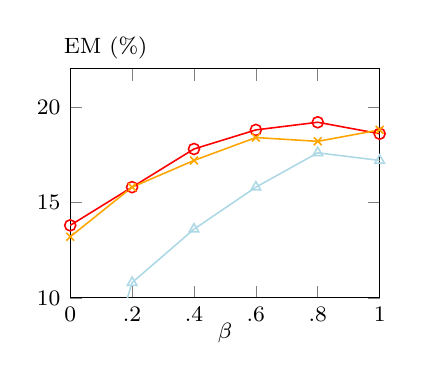
\begin{tikzpicture}[scale=1]
    \begin{axis}[
        height=\columnwidth/2.7,
        width=\columnwidth/2.2,
        ylabel={EM (\%)},
        xlabel={$\beta$},
        xmin=0.0, xmax=1.0,
        ymin=0.1, ymax=0.22,
        xtick={0, 0.2, 0.4, 0.6, 0.8, 1.0},
        xticklabel style = {font=\footnotesize},
        xticklabels={0, .2, .4, .6, .8, 1},
        ytick={0.1, 0.15, 0.2},
        yticklabels={10, 15, 20},
        every axis y label/.style={at={(current axis.north west)},right=4.5mm,above=0mm},
        label style={font=\footnotesize},
        tick label style={font=\footnotesize},
        every axis x label/.style={at={(current axis.south)},right=0mm,above=-7mm},
        label style={font=\footnotesize},
        tick label style={font=\footnotesize},
    ]

%     \addplot[line width=0.2mm,mark size=2pt,mark=o,color=Red]
%         plot coordinates { % SkeTRAG
% (0, 0.122)
% (0.2, 0.132)
% (0.4, 0.144)
% (0.6, 0.134)
% (0.8, 0.14)
% (1.0, 0.114)
%     };

%     \addplot[line width=0.2mm,mark size=2pt,mark=o,color=Red!75]
%         plot coordinates { % SkeTRAG - 600
% (0, 0.108)
% (0.2, 0.174)
% (0.4, 0.17)
% (0.6, 0.172)
% (0.8, 0.166)
% (1.0, 0.152)
%     };

%     \addplot[line width=0.2mm,mark size=2pt,mark=o,color=Red!50]
%         plot coordinates { % SkeTRAG - 300
% (0, 0.104)
% (0.2, 0.176)
% (0.4, 0.192)
% (0.6, 0.186)
% (0.8, 0.198)
% (1.0, 0.192)
%     };

    \addplot[line width=0.2mm,mark size=2pt,mark=o,color=Red]
        plot coordinates { % SkeTRAG - 150
(0.0, 0.138)
(0.2, 0.158)
(0.4, 0.178)
(0.6, 0.188)
(0.8, 0.192)
(1.0, 0.186)
    };

    \addplot[line width=0.2mm,mark size=2pt,mark=x,color=Orange]
        plot coordinates { % SkeTRAG - uniform
(0.0, 0.132)
(0.2, 0.158)
(0.4, 0.172)
(0.6, 0.184)
(0.8, 0.182)
(1.0, 0.188)
    };

%     \addplot[line width=0.2mm,mark size=2pt,mark=star,color=DeepBlue]
%         plot coordinates { % skeleton - uniform
% (0.0, 0.0)
% (0.2, 0.106)
% (0.4, 0.132)
% (0.6, 0.164)
% (0.8, 0.174)
% (1.0, 0.174)
%     };


    \addplot[line width=0.2mm,mark size=2pt,mark=triangle,color=LightBlue]
        plot coordinates { % skeleton
(0.0, 0.0)
(0.2, 0.108)
(0.4, 0.136)
(0.6, 0.158)
(0.8, 0.176)
(1.0, 0.172)
    };
    
    \end{axis}

\end{tikzpicture}
\hspace{-1.2mm}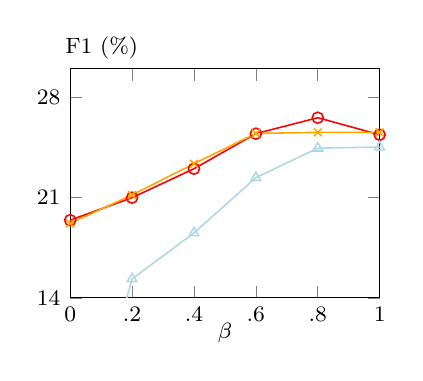
\begin{tikzpicture}[scale=1]
    \begin{axis}[
        height=\columnwidth/2.7,
        width=\columnwidth/2.2,
        ylabel={F1 (\%)},
        xlabel={$\beta$},
        xmin=0.0, xmax=1.0,
        ymin=0.14, ymax=0.3,
        xtick={0, 0.2, 0.4, 0.6, 0.8, 1.0},
        xticklabel style = {font=\footnotesize},
        xticklabels={0, .2, .4, .6, .8, 1},
        ytick={0.14, 0.21, 0.28},
        yticklabels={14, 21, 28},
        every axis y label/.style={at={(current axis.north west)},right=4mm,above=0mm},
        label style={font=\footnotesize},
        tick label style={font=\footnotesize},
        every axis x label/.style={at={(current axis.south)},right=0mm,above=-7mm},
        label style={font=\footnotesize},
        tick label style={font=\footnotesize},
    ]

%     \addplot[line width=0.2mm,mark size=2pt,mark=o,color=Red]
%         plot coordinates { % SkeTRAG - 1200
% (0, 0.176300934)
% (0.2, 0.188094157)
% (0.4, 0.196128801)
% (0.6, 0.1876783)
% (0.8, 0.19700453)
% (1.0, 0.157561628)
%     };

%     \addplot[line width=0.2mm,mark size=2pt,mark=o,color=Red!75]
%         plot coordinates { % SkeTRAG - 600
% (0, 0.170179462)
% (0.2, 0.240968426)
% (0.4, 0.226319961)
% (0.6, 0.232188549)
% (0.8, 0.229216351)
% (1.0, 0.208775333)
%     };

%     \addplot[line width=0.2mm,mark size=2pt,mark=o,color=Red!50]
%         plot coordinates { % SkeTRAG - 300
% (0, 0.169292118)
% (0.2, 0.24154141)
% (0.4, 0.256892671)
% (0.6, 0.255549124)
% (0.8, 0.266975679)
% (1.0, 0.256770818)
%     };

    \addplot[line width=0.2mm,mark size=2pt,mark=o,color=Red]
        plot coordinates { % SkeTRAG - 150
(0.0, 0.194302287)
(0.2, 0.209992062)
(0.4, 0.23021343)
(0.6, 0.254704947)
(0.8, 0.265845586)
(1.0, 0.253952005)
    };

    \addplot[line width=0.2mm,mark size=2pt,mark=x,color=Orange]
        plot coordinates { % SkeTRAG - uniform
(0.0, 0.192066627)
(0.2, 0.211880355)
(0.4, 0.233691958)
(0.6, 0.254856333)
(0.8, 0.255602241)
(1.0, 0.255616111)
    };

    \addplot[line width=0.2mm,mark size=2pt,mark=triangle,color=LightBlue]
        plot coordinates { % skeleton
(0.0, 0.0)
(0.2, 0.153266376)
(0.4, 0.185392483)
(0.6, 0.223946198)
(0.8, 0.244550107)
(1.0, 0.245370649)
    };

%     \addplot[line width=0.2mm,mark size=2pt,mark=star,color=DeepBlue]
%         plot coordinates { % skeleton - uniform
% (0.0, 0.0)
% (0.2, 0.148484271)
% (0.4, 0.200356146)
% (0.6, 0.235926157)
% (0.8, 0.247588566)
% (1.0, 0.247293046)
%     };

\end{axis}

\end{tikzpicture}
}%
\\
\subfloat[Hotpot]{
\hspace{-1.2mm}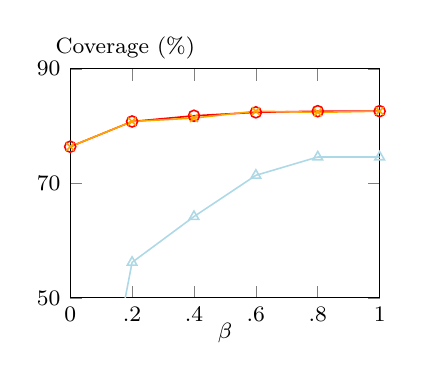
\begin{tikzpicture}[scale=1]
    \begin{axis}[
        height=\columnwidth/2.7,
        width=\columnwidth/2.2,
        ylabel={Coverage (\%)},
        xlabel={$\beta$},
        xmin=0.0, xmax=1.0,
        ymin=0.5, ymax=0.9,
        xtick={0, 0.2, 0.4, 0.6, 0.8, 1.0},
        xticklabel style = {font=\footnotesize},
        xticklabels={0, .2, .4, .6, .8, 1},
        ytick={0.5, 0.7, 0.9},
        yticklabels={50, 70, 90},
        every axis y label/.style={at={(current axis.north west)},right=7mm,above=0mm},
        label style={font=\footnotesize},
        tick label style={font=\footnotesize},
        every axis x label/.style={at={(current axis.south)},right=0mm,above=-7mm},
        label style={font=\footnotesize},
        tick label style={font=\footnotesize},
    ]

    \addplot[line width=0.2mm,mark size=2pt,mark=o,color=Red]
        plot coordinates { % SkeTRAG - 150
(0.0, 0.764)
(0.2, 0.808)
(0.4, 0.818)
(0.6, 0.824)
(0.8, 0.826)
(1.0, 0.826)
    };

    \addplot[line width=0.2mm,mark size=2pt,mark=x,color=Orange]
        plot coordinates { % SkeTRAG - uniform
(0.0, 0.764)
(0.2, 0.808)
(0.4, 0.814)
(0.6, 0.826)
(0.8, 0.824)
(1.0, 0.826)
    };

    \addplot[line width=0.2mm,mark size=2pt,mark=triangle,color=LightBlue]
        plot coordinates { % skeleton
(0.0, 0.0)
(0.2, 0.562)
(0.4, 0.642)
(0.6, 0.714)
(0.8, 0.746)
(1.0, 0.746)
    };

%     \addplot[line width=0.2mm,mark size=2pt,mark=star,color=DeepBlue]
%         plot coordinates { % skeleton - uniform
% (0.0, 0.0)
% (0.2, 0.576)
% (0.4, 0.686)
% (0.6, 0.732)
% (0.8, 0.736)
% (1.0, 0.746)
%     };
    \end{axis}

\end{tikzpicture}
\hspace{-1.2mm}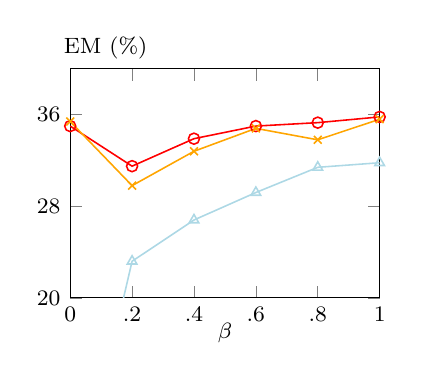
\begin{tikzpicture}[scale=1]
    \begin{axis}[
        height=\columnwidth/2.7,
        width=\columnwidth/2.2,
        ylabel={EM (\%)},
        xlabel={$\beta$},
        xmin=0.0, xmax=1.0,
        ymin=0.2, ymax=0.4,
        xtick={0, 0.2, 0.4, 0.6, 0.8, 1.0},
        xticklabel style = {font=\footnotesize},
        xticklabels={0, .2, .4, .6, .8, 1},
        ytick={0.2, 0.28, 0.36},
        yticklabels={20, 28, 36},
        every axis y label/.style={at={(current axis.north west)},right=4.5mm,above=0mm},
        label style={font=\footnotesize},
        tick label style={font=\footnotesize},
        every axis x label/.style={at={(current axis.south)},right=0mm,above=-7mm},
        label style={font=\footnotesize},
        tick label style={font=\footnotesize},
    ]

    \addplot[line width=0.2mm,mark size=2pt,mark=o,color=Red]
        plot coordinates { % SkeTRAG - 150
(0.0, 0.35)
(0.2, 0.315)
(0.4, 0.339)
(0.6, 0.35)
(0.8, 0.353)
(1.0, 0.358)
    };

    \addplot[line width=0.2mm,mark size=2pt,mark=x,color=Orange]
        plot coordinates { % SkeTRAG - uniform
(0.0, 0.354)
(0.2, 0.298)
(0.4, 0.328)
(0.6, 0.348)
(0.8, 0.338)
(1.0, 0.356)
    };

    \addplot[line width=0.2mm,mark size=2pt,mark=triangle,color=LightBlue]
        plot coordinates { % skeleton
(0.0, 0.0)
(0.2, 0.232)
(0.4, 0.268)
(0.6, 0.292)
(0.8, 0.314)
(1.0, 0.318)
    };

%     \addplot[line width=0.2mm,mark size=2pt,mark=star,color=DeepBlue]
%         plot coordinates { % skeleton - uniform
% (0.0, 0.0)
% (0.2, 0.204)
% (0.4, 0.302)
% (0.6, 0.318)
% (0.8, 0.326)
% (1.0, 0.318)
%     };
    
    \end{axis}

\end{tikzpicture}
\hspace{-1.2mm}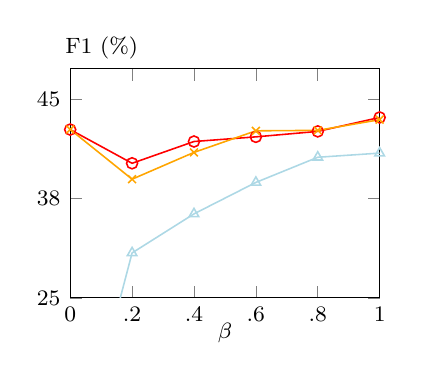
\begin{tikzpicture}[scale=1]
    \begin{axis}[
        height=\columnwidth/2.7,
        width=\columnwidth/2.2,
        ylabel={F1 (\%)},
        xlabel={$\beta$},
        xmin=0.0, xmax=1.0,
        ymin=0.25, ymax=0.55,
        xtick={0, 0.2, 0.4, 0.6, 0.8, 1.0},
        xticklabel style = {font=\footnotesize},
        xticklabels={0, .2, .4, .6, .8, 1},
        ytick={0.25,0.38, 0.51},
        yticklabels={25, 38, 45, 51},
        every axis y label/.style={at={(current axis.north west)},right=4mm,above=0mm},
        label style={font=\footnotesize},
        tick label style={font=\footnotesize},
        every axis x label/.style={at={(current axis.south)},right=0mm,above=-7mm},
        label style={font=\footnotesize},
        tick label style={font=\footnotesize},
    ]

    \addplot[line width=0.2mm,mark size=2pt,mark=o,color=Red]
        plot coordinates { % SkeTRAG - 150
(0.0, 0.470434704)
(0.2, 0.426276111)
(0.4, 0.454788870)
(0.6, 0.460886061)
(0.8, 0.468036694)
(1.0, 0.486306113)
    };

    \addplot[line width=0.2mm,mark size=2pt,mark=x,color=Orange]
        plot coordinates { % SkeTRAG - uniform
(0.0, 0.470574266)
(0.2, 0.405430301)
(0.4, 0.44053814)
(0.6, 0.468784679)
(0.8, 0.469378725)
(1.0, 0.483362192)
    };

    \addplot[line width=0.2mm,mark size=2pt,mark=triangle,color=LightBlue]
        plot coordinates { % skeleton
(0.0, 0.0)
(0.2, 0.308885359)
(0.4, 0.360015033)
(0.6, 0.401194074)
(0.8, 0.434159393)
(1.0, 0.439605784)
    };

%     \addplot[line width=0.2mm,mark size=2pt,mark=star,color=DeepBlue]
%         plot coordinates { % skeleton - uniform
% (0.0, 0.0)
% (0.2, 0.282341829)
% (0.4, 0.394474657)
% (0.6, 0.430782795)
% (0.8, 0.434493561)
% (1.0, 0.438056246)
%     };
    
    \end{axis}

\end{tikzpicture}
}%
\vspace{-2mm}
\caption{Answer quality by varying $\beta$.} \label{fig:quality-beta}
\vspace{-4mm}
\end{figure}